\section{Work Breakdown Structure}

\begin{figure}[H]
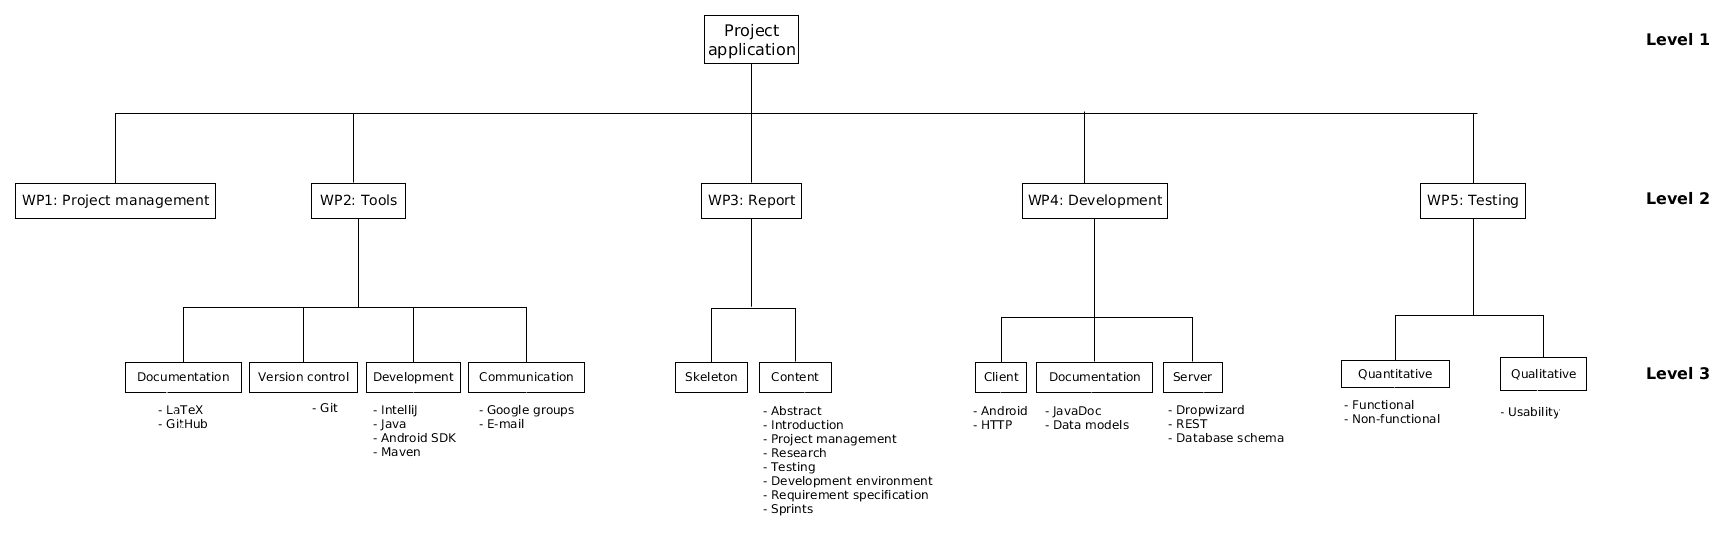
\includegraphics[width=\textwidth]{ch/prestudy/fig/wbs.png}
\caption{Product oriented work breakdown structure for the project application.}
\label{fig:wbs}
\end{figure}

As shown in figure~\ref{fig:wbs}, the Work Breakdown Structure (WBS) is divided into five work packages(WP). Each work package represents a subset of the project. Specifically, it specifies \emph{what} will be done, and not how or when the work is to be performed.

The team used WBS in order to get an overview of what kind of work the different parts of the project consisted of, and used this information when we estimated how much time we wanted to use on each work package.

The estimated time for each work package is given in table~\ref{tab:timeEstWP}. By comparing the original time estimates to how much time that actually was spent, we were able to evaluate our project's progress to a much greater extent. It was easier to see whether some part of the project was forgotten, and if it should have been estimated more, or less, time to complete.

\begin{table}[H]
\centering
\rowcolors{1}{darkgray}{lightgray}
\begin{tabular}{|l|c|c|r|}
\hline
    \textbf{WP \#} & \textbf{Name} & \textbf{Percentage} & \textbf{Hours} \\\hline
    1 & Project management & 5 & 87\\\hline
    2 & Tools 			   & 15 & 261\\\hline
    3 & Report 			   & 40 & 696\\\hline
    4 & Development 	   & 30 & 522\\\hline
    5 & Testing  		   & 10 & 174\\\hline
\end{tabular}
\caption{Time estimate for work packages}
\label{tab:timeEstWP}
\end{table}